\documentclass[12pt]{beamer}
\usetheme{CambridgeUS}
\usepackage[utf8]{inputenc}
\usepackage[german]{babel}
\usepackage[T1]{fontenc}
\usepackage{amsmath}
\usepackage{amsfonts}
\usepackage{amssymb}
\usepackage{graphicx}

\author{Philipp Hörauf und Toni Bartsch}
\title{DIY: Carbonwickelmaschine}

\setbeamercovered{transparent} 
%\setbeamertemplate{navigation symbols}{} 
%\logo{}  %Dickbutt!
%\institute{} 
\date{\today} 
%\subject{} 

\begin{document}


\begin{frame}
\titlepage
\end{frame}


\begin{frame}
\tableofcontents
\end{frame}


\begin{frame}{Motivation}
toller satz...\newline
\vspace{1cm}
\pause
Carbonrohre sind...
\begin{itemize}
	\item<1-> extrem leicht
	\item<2-> verwindungssteif
	\item<3-> korrosionsbeständig
	\item<4-> quasi immun gegen Wärmeausdehnung
\end{itemize}
\vspace*{1cm}
\pause 
Daher ist Carbon ideal für leichte und zugleich robuste Aufbauten geeignet, z.B. im Modellbau
\end{frame}


\begin{frame}
Problem: Carbonrohre können teuer werden, vor allem wenn man größere Mengen oder exotische Maße benötigt.\newline

\begin{figure}
	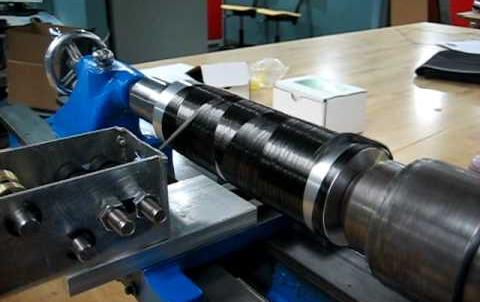
\includegraphics[width=6cm]{./hqdefault.jpg}
	\caption{professionelle Carbonwickelmaschine, \url{http://carbon-deutschland.de}}
\end{figure}

Diese Maschinen sind recht teuer und schwer erhältlich.
\end{frame}


\begin{frame}{Projektbeschreibung}
Daher: Eigenbau einer Carbonwickelmaschine aus Normteilen und selbst designtem.\newline
\vspace{0.5cm}

\pause
voraussichtliche Eckdaten der Maschine:
\begin{itemize}
	\item<1-> Maximale Wickellänge 1200\,mm
	\item<2-> Größter Durchmesser 250\,mm
	\item<3-> Verarbeitung von Carbon- und Glasfasern
	\item<4-> Wickelvorgang PC-kontrolliert
	\item<5-> Möglichst kostengünstiger Aufbau
\end{itemize}
\end{frame}


\end{document}